
\chapter{Application: international trade}

\section{The determinants of trade}

Consider the market for steel.
We examine here the steel market in the imaginary country of Isoland.


\subsection{The equilibrium without trade}


Because there is no international trade, the market for steel in Isoland consists solely of Isolandian buyers and sellers.
As Figure \ref{fig:equilibrium-without-international-trade} shows, the domestic price adjusts to balance the quantity supplied by domestic sellers and the quantity demanded by domestic buyers.

\begin{figure}[!ht]
  \centering
  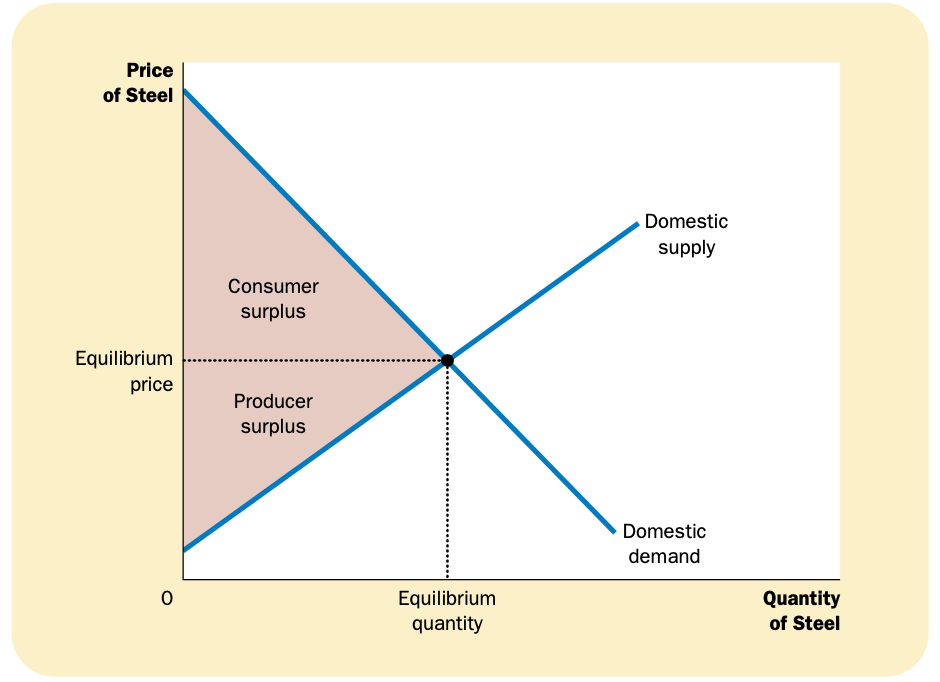
\includegraphics[width=\textwidth]{pics/the-equilibrium-without-international-trade}
  \caption{The equilibrium without trade}
  \label{fig:equilibrium-without-international-trade}
\end{figure}



\keyword{world price}: the price of a good that prevails in the world market for that good.


\section{The winners and losers from trade}

\subsection{The gains and losses of an exporting country}

Figure \ref{fig:international-trade-in-an-exporting-country} shows the Isolandian steel market when the domestic equilibrium price before trade is below the world price.

\begin{figure}[!ht]
  \centering
  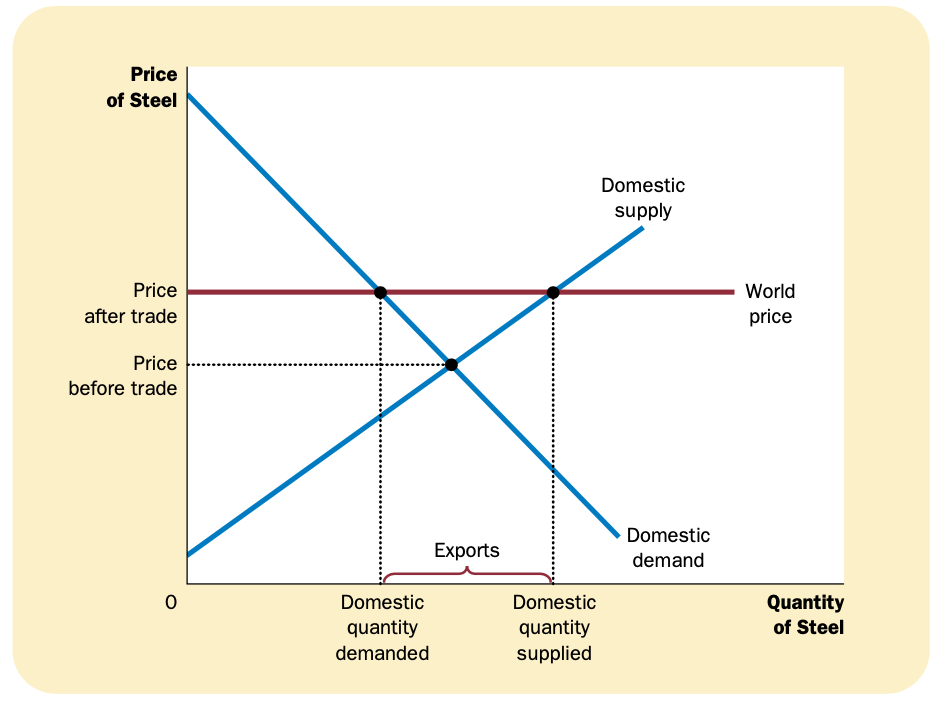
\includegraphics[width=\textwidth]{pics/international-trade-in-an-exporting-country}
  \caption{International trade in an exporting country}
  \label{fig:international-trade-in-an-exporting-country}
\end{figure}


Clearly, not everyone benefits. Trade forces the domestic price to rise to the world price. Domestic producers of steel are better off because they can now sell steel at a higher price, but domestic consumers of steel are worse off because they have to buy steel at a higher price.


To measure these gains and losses, we look at the changes in consumer and producer surplus, which are shown in Figure \ref{fig:how-free-trade-affects-walfare-in-an-exporting-country}.


\begin{figure}[!ht]
  \centering
  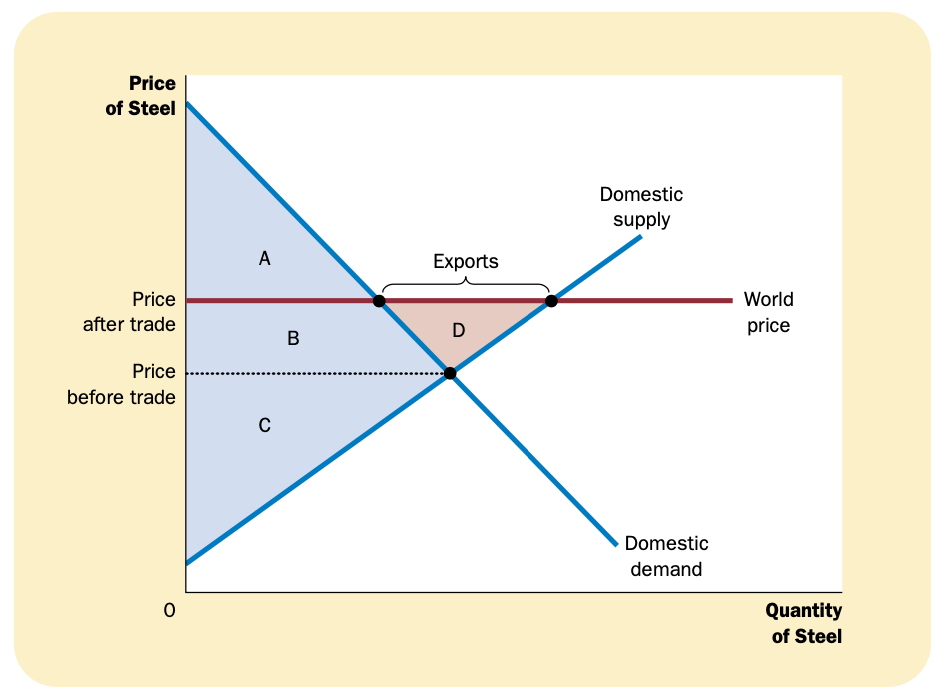
\includegraphics[width=\textwidth]{pics/how-free-trade-affects-walfare-in-an-exporting-country}
  \caption{How free trade affects welfare in an exporting country}
  \label{fig:how-free-trade-affects-walfare-in-an-exporting-country}
\end{figure}


These welfare calculations show who wins and who loses from trade in an exporting country. Sellers benefit because producer surplus increases by the area $B+D$. Buyers are worse off because consumer surplus decreases by the area B. Because the gains of sellers exceed the losses of buyers by the area D, total surplus in Isoland increases.



This analysis of an exporting country yields two conclusions:
\begin{enumerate}
\item When a country allows trade and becomes an exporter of a good, domestic producers of the good are better off, and domestic consumers of the good are worse off.
\item Trade raises the economic well-being of a nation in the sense that the gains of the winners exceed the losses of the losers.
\end{enumerate}



\subsection{The gains and losses of an importing country}

Figure \ref{fig:international-trade-in-an-exporting-country} show the situation.

\begin{figure}[!ht]
  \centering
  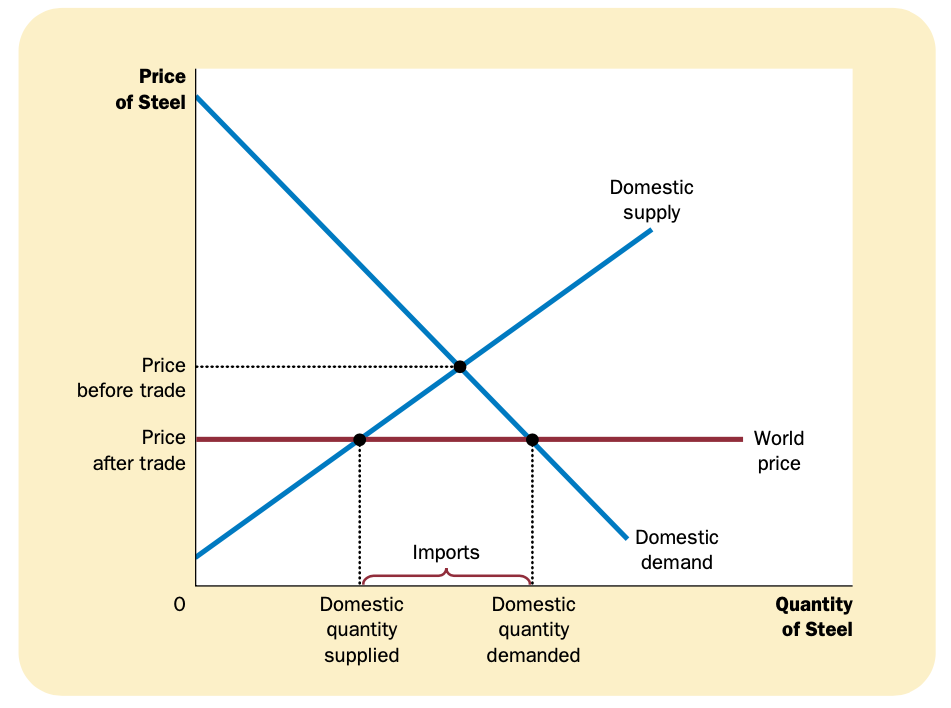
\includegraphics[width=\textwidth]{pics/international-trade-in-an-importing-country}
  \caption{International trade in an importing country}
  \label{fig:internaltional-trade-in-an-importing-country}
\end{figure}



Now consider the gains and losses from trade. Once again, not everyone benefits. When trade forces the domestic price to fall, domestic consumers are better off (they can now buy steel at a lower price), and domestic producers are worse off (they now have to sell steel at a lower price). Changes in consumer and producer surplus measure the size of the gains and losses, as shown in Figure \ref{fig:how-free-trade-affects-welfare-in-an-importing-country}.

\begin{figure}[!ht]
  \centering
  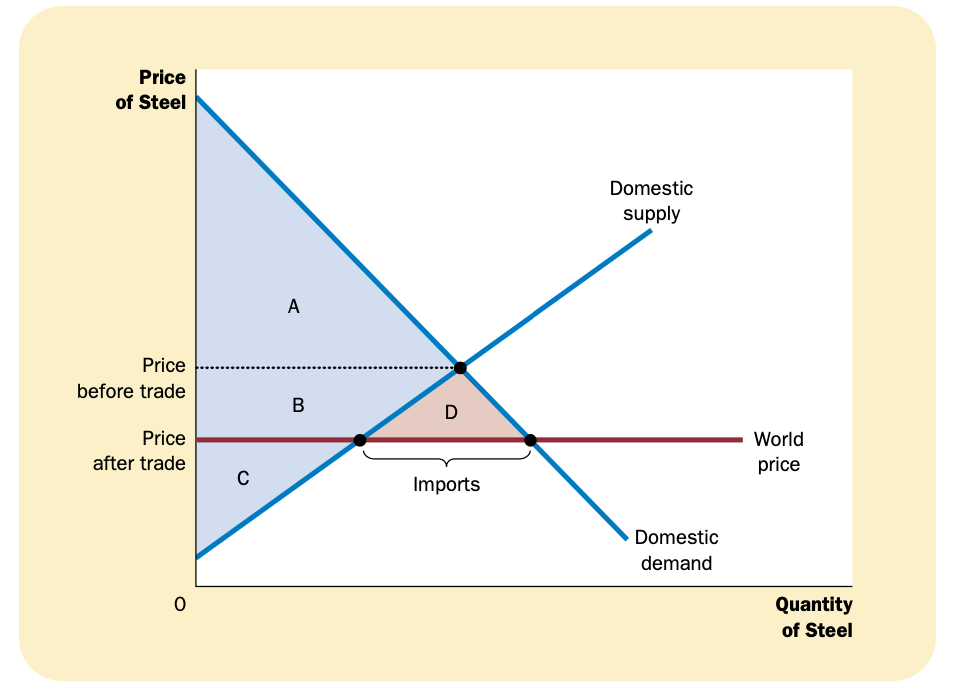
\includegraphics[width=\textwidth]{pics/how-free-trade-affects-welfare-in-an-importing-country}
  \caption{How free trade affects welfare in an importing country}
  \label{fig:how-free-trade-affects-welfare-in-an-importing-country}
\end{figure}


Buyers benefit because consumer surplus increases by the area $B+D$. Sellers are worse off because producer surplus falls by the area B. The gains of buyers exceed the losses of sellers, and total surplus increases by the area D.


This analysis of an importing country yields two conclusions parallel to those for an exporting country:
\begin{enumerate}
\item When a country allows trade and becomes an importer of a good, domestic consumers of the good are better off, and domestic producers of the good are worse off.
\item Trade raises the economic well-being of a nation in the sense that the gains of the winners exceed the losses of the losers.
\end{enumerate}


\subsection{The effects of a tariff}

The economists quickly realize that a tariff on steel will have no effect if Isoland becomes a steel exporter.
If no one in Isoland is interested in importing steel, a tax on steel imports is irrelevant.
The tariff matters only if Isoland becomes a steel importer.



Figure \ref{fig:the-effect-of-a-tariff} shows the Isolandian market for steel.

\begin{figure}[!ht]
  \centering
  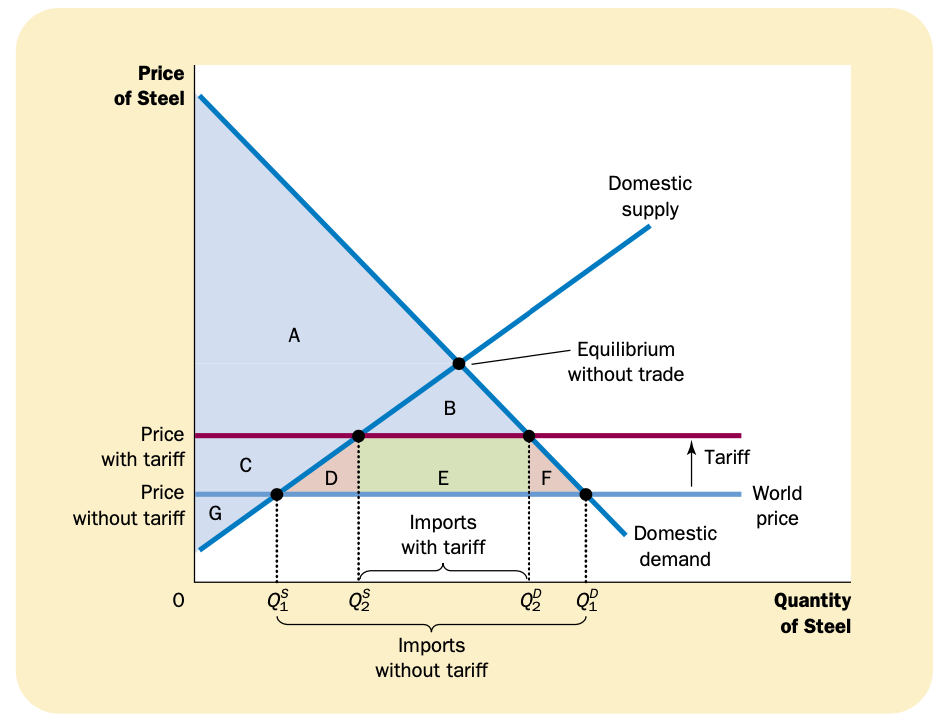
\includegraphics[width=\textwidth]{pics/the-effect-of-a-tariff}
  \caption{The effect of a tariff}
  \label{fig:the-effect-of-a-tariff}
\end{figure}


The change in price affects the behavior of domestic buyers and sellers.
Because the tariff raises the price of steel, it reduces the domestic quantity demanded from $Q_1^D $ to $Q_2^D$ and raises the domestic quantity supplied from $Q_1^S$ to $Q_2^S$.
Thus, \keyword{the tariff reduces the quantity of imports and moves the domestic market closer to its equilibrium without trade}.



The comparison before and after the tariff is shown in \ref{fig:changes-in-welfare-from-a-tariff}.

\begin{figure}[!ht]
  \centering
  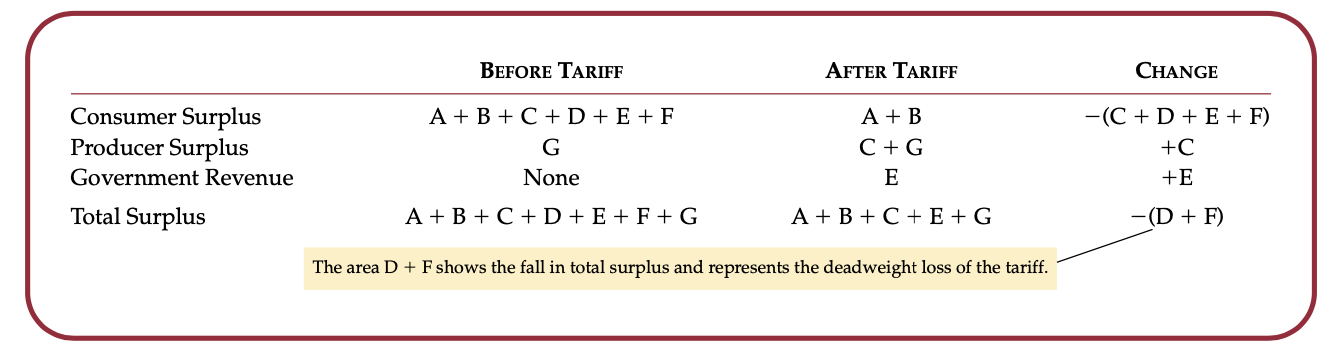
\includegraphics[width=\textwidth]{pics/changes-in-welfare-from-a-tariff}
  \caption{Changes in welfare from a tariff}
  \label{fig:changes-in-welfare-from-a-tariff}
\end{figure}



\subsection{The effect of an import quota}

\keyword{import quota}: a limit on the quantity of a good that can be produced abroad and sold domestically.


Imagine that the Isolandian government distributes a limited number of import licenses. Each license gives the license holder the right to import 1 ton of steel into Isoland from abroad.
Figure \ref{fig:the-effect-of-an-important-quota} shows how an important quota affects the Isolandian market for steel.

\begin{figure}[!ht]
  \centering
  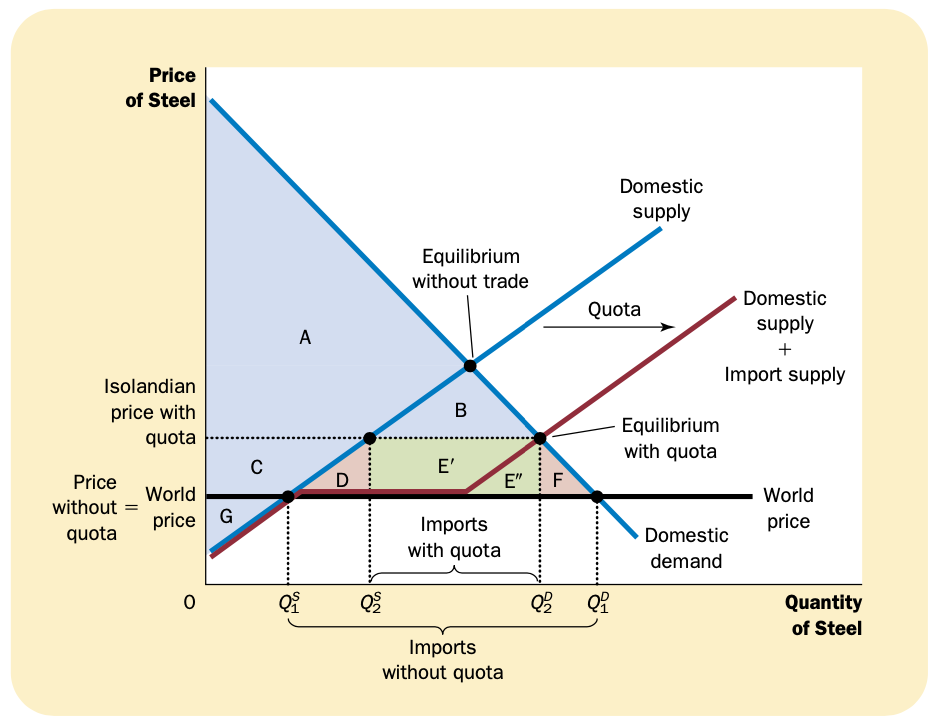
\includegraphics[width=\textwidth]{pics/the-effect-of-an-import-quota}
  \caption{The effect of an important quota}
  \label{fig:the-effect-of-an-important-quota}
\end{figure}


\begin{figure}[!ht]
  \centering
  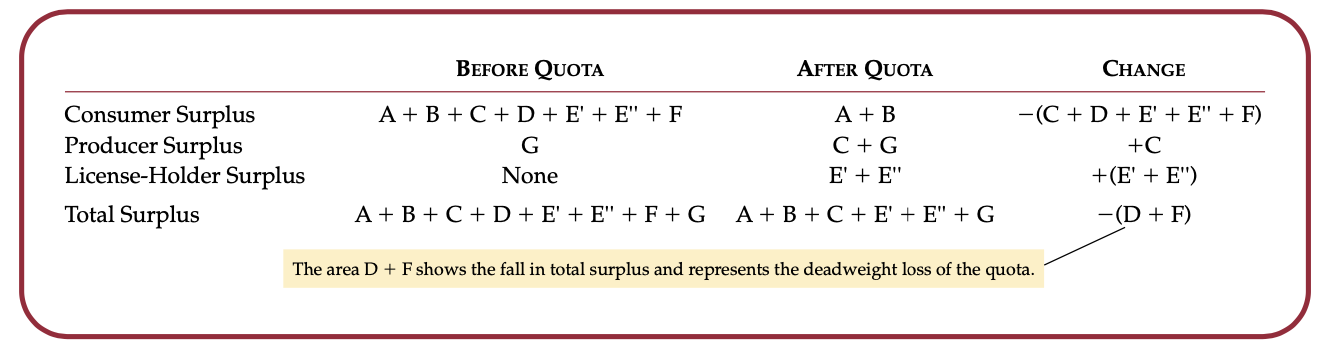
\includegraphics[width=\textwidth]{pics/changes-in-welfare-from-an-import-quota}
  \caption{Changes in welfare from an import quota}
  \label{fig:changes-in-welfare-from-an-import-quota}
\end{figure}

The changes is shown in table \ref{fig:changes-in-welfare-from-an-import-quota}.


Both tariffs and import quotas raise the domestic price of the good, reduce the welfare of domestic consumers, increase the welfare of domestic producers, and cause deadweight losses.





